\documentclass[14pt,xcolor=dvipsnames,table,dvipdfmx]{beamer}

\setbeamertemplate{bibliography item}[text]
\usepackage[absolute,overlay]{textpos}

\usetheme{Boadilla}

\usepackage{txfonts} % TXフォント
\renewcommand{\kanjifamilydefault}{\gtdefault}  % 日本語をゴシック体に
\usefonttheme{structurebold} % タイトル部を太字
\setbeamerfont{alerted text}{series=\bfseries} % Alertを太字
\setbeamerfont{section in toc}{series=\mdseries} % 目次は太字にしない
\setbeamerfont{frametitle}{size=\Large} % フレームタイトル文字サイズ
\setbeamerfont{title}{size=\LARGE} % タイトル文字サイズ
\setbeamerfont{date}{size=\small}  % 日付文字サイズ
\usepackage{pxjahyper}

\uselanguage{japanese}
\languagepath{japanese}
\deftranslation[to=japanese]{Theorem}{定理}
\deftranslation[to=japanese]{Lemma}{補題}
\deftranslation[to=japanese]{Example}{例}
\deftranslation[to=japanese]{Examples}{例}
\deftranslation[to=japanese]{Definition}{定義}
\deftranslation[to=japanese]{Definitions}{定義}
\deftranslation[to=japanese]{Problem}{問題}
\deftranslation[to=japanese]{Solution}{解}
\deftranslation[to=japanese]{Fact}{事実}
\deftranslation[to=japanese]{Proof}{証明}
\def\proofname{証明}

\definecolor{UniBlue}{RGB}{0,150,200} 
\definecolor{AlertOrange}{RGB}{255,76,0}
\definecolor{AlmostBlack}{RGB}{38,38,38}
\setbeamercolor{normal text}{fg=AlmostBlack}  % 本文カラー
\setbeamercolor{structure}{fg=UniBlue} % 見出しカラー
\setbeamercolor{block title}{fg=UniBlue!50!black} % ブロック部分タイトルカラー
\setbeamercolor{alerted text}{fg=AlertOrange} % \alert 文字カラー
\mode<beamer>{
    \definecolor{BackGroundGray}{RGB}{254,254,254}
    \setbeamercolor{background canvas}{bg=BackGroundGray} % スライドモードのみ背景をわずかにグレーにする
}

%フラットデザイン化
\setbeamertemplate{blocks}[rounded] % Blockの影を消す
\useinnertheme{circles} % 箇条書きをシンプルに
\setbeamertemplate{navigation symbols}{} % ナビゲーションシンボルを消す
\setbeamertemplate{footline}[frame number] % フッターはスライド番号のみ

\AtBeginSection[]{
    \frame{\tableofcontents[currentsection, hideallsubsections]} %目次スライド
}

\title{\bfseries Private Information Retrieval}
%\subtitle{\bfseries ─ 講演用スライド作成のために ─}
\author{胡瀚林}
\date{\today}
%\institute{東京電機大学工学部 物理系列}
%\subject{PIR}
%\keywords{PIR,Obfuscation,query}

\begin{document}

\maketitle
\frame{\tableofcontents[hideallsubsections]}

\section{背景}
\begin{frame}{Private Information Retrieval}

\begin{columns}[t]
    \begin{column}{0.8\textwidth} % 横幅の30%
      	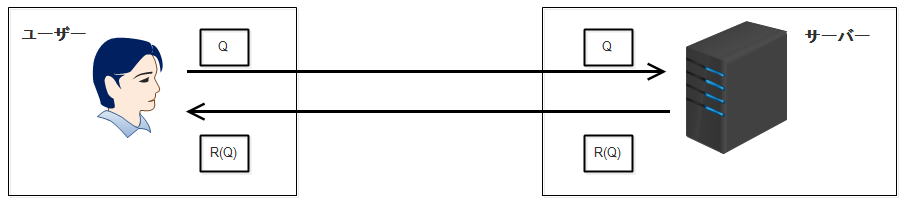
\includegraphics[width=\columnwidth]{photo1.png}
    \end{column}
\end{columns}
	\begin{block}{}
	\begin{itemize}
    	\item Q:検索質問
		\item R(Q):質問Qの検索結果
	\end{itemize}
	\end{block}
\end{frame}

\begin{frame}{Location vs Keyword}
	\begin{block}{}
		\begin{itemize}
		\item Location
			\begin{itemize}
			\item 地図
			\item 乗換案内
			\item 近くのラストラン
			\end{itemize}
		\end{itemize}
        \begin{itemize}
        \item Keyword
            \begin{itemize}
            \item ウェブ検索
            \item データベース検索
            \item クラウドストア検索
            \end{itemize}
        \end{itemize}
	\end{block}
\end{frame}

\begin{frame}{AOL 事件}
	\begin{exampleblock}{AOL質問ログ}
	\fontsize{7pt}{7.2}\selectfont
	\begin{tabular}{ccccc}
	\noalign{\hrule height 1pt}
	AnonID & Query & QueryTime & ItemRank & ClickURL \\
	\hline
	4417749 & care packages & 2006-03-02 09:19:32 & 10 & http://booksforsoldiers.com \\
 	4417749 & care packages & 2006-03-02 09:19:32 & 9 & http://www.brandonblog.com \\
	4417749 & movies for dogs & 2006-03-02 09:24:14 & & \\		
	4417749 & blue book & 2006-03-03 11:48:52 & 1 & http://www.kbb.com \\
	4417749 & best dog for older owner & 2006-03-06 11:48:24 & 1 & http://www.canismajor.com \\
	4417749 & best dog for older owner & 2006-03-06 11:48:24 & 5 & http://dogs.about.com \\
	\noalign{\hrule height 1pt}
	\end{tabular}
	\end{exampleblock}
	\begin{block}{}
	\begin{itemize}
		\item 2006年8月4日、AOL(American OnLine)が650,000人以上のユーザーの匿名化された検索質問ログを研究目的でリリースした。\pause
		\item 2006年8月9日、ID 4417749の名前、年齢、住所などが特定された。\cite{AOL}
	\end{itemize}
	\end{block}
\end{frame}

\begin{frame}
\end{frame}

\section{守り方}
\begin{frame}{Anonymity}
\begin{columns}[t]
    \begin{column}{0.8\textwidth} % 横幅の30%
        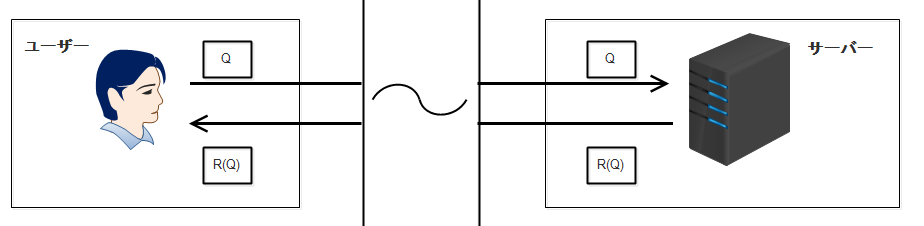
\includegraphics[width=\columnwidth]{photo2.png}
    \end{column}
\end{columns}

\end{frame}
\begin{frame}{Obfuscation}
\end{frame}
\begin{frame}{PIR}
\end{frame}
\begin{frame}{Obfuscation + PIR}
\end{frame}


\section{攻撃方}
\begin{frame}
\end{frame}
\begin{frame}
\end{frame}
\begin{frame}
\end{frame}


\begin{frame}[t,allowframebreaks]{Bibliography}
\bibliographystyle{siam}
\bibliography{zotero}
\end{frame}

\end{document}
